\chapter{The lattice laboratory and the six-current embedding}
\label{ch:lattice_embedding}

An existence problem becomes much more manageable when the proposed fields
already live in a known theory. Their products then have meanings before we
try to recognize the algebra they generate. In this chapter we construct
the laboratory for the Haagerup example: an eight-dimensional lattice
theory, two commuting affine current algebras, and a particular field of
weight two. The calculations require the state--field correspondence,
Heisenberg oscillators, and the elementary representation theory of
$\mathfrak{sl}_2$. Our aim is to see where the special numbers $13$ and
$39$ enter, and to understand precisely what has, and has not, been
constructed when the generators have been written down.

\section{From a positive lattice to fields}
\index{lattice vertex algebra}\index{cocycle!lattice signs}

Let $L$ be a positive-definite even integral lattice. Integral means that
$(\alpha,\beta)\in\Z$ for $\alpha,\beta\in L$; even means that
$(\alpha,\alpha)\in2\Z$. The vector space of its lattice vertex algebra is
\begin{equation}\label{eq:c-lattice-space}
 V_L=S\bigl(\mathfrak h\otimes t^{-1}\C[t^{-1}]\bigr)
          \otimes\C_\epsilon[L],\qquad
 \mathfrak h=L\otimes_\Z\C.
\end{equation}
Here $S$ denotes the symmetric algebra of the negative oscillator modes,
so the first factor is an oscillator Fock space. The second has one basis
vector $e^\alpha$ for each lattice momentum, with multiplication
$e^\alpha e^\beta=\epsilon(\alpha,\beta)e^{\alpha+\beta}$.
The symbol $\epsilon$ records a sign convention. It is needed
because the exponential fields have to be mutually local, including
their signs.

A typical basis vector has the form
\[
 h_1(-n_1)\cdots h_r(-n_r)e^\alpha,
 \qquad n_i\geq1,
\]
and its conformal weight is
\begin{equation}\label{eq:c-lattice-grade}
 \frac{(\alpha,\alpha)}2+n_1+\cdots+n_r.
\end{equation}
Thus the weight is nonnegative and integral. Positive definiteness is
doing two jobs: it bounds the possible momenta at fixed weight, and it
makes the natural Hilbert-space form positive. Neither statement would
remain automatic for an indefinite lattice.

For the root lattice used below, choose a simple-root basis
$\alpha_0,\ldots,\alpha_7$ with Gram matrix $G$ and $G_{ii}=2$.
We use the following concrete cocycle in this basis:
\begin{equation}\label{eq:c-lattice-cocycle}
 \epsilon(a,b)=(-1)^{\sum_i a_i b_i+
                           \sum_{i>j}a_i b_jG_{ij}}.
\end{equation}
Its exponent is bilinear modulo two, so associativity of the twisted
group algebra follows immediately. The identities
\[
 \frac{\epsilon(a,b)}{\epsilon(b,a)}=(-1)^{(a,b)},
 \qquad \epsilon(a,-a)=(-1)^{(a,a)/2}
\]
are useful sign checks. They show explicitly how the lattice pairing
controls locality. For a general even lattice basis, the diagonal
contribution $\sum_i a_i b_i$ must be replaced by
$\sum_i(G_{ii}/2)a_i b_i$; the root-basis formula is not a
basis-independent prescription.

For a pure momentum state, the part of the vertex operator that acts on
another pure momentum state is
\begin{equation}\label{eq:c-lattice-product}
 Y(e^a,z)e^b=\epsilon(a,b)z^{(a,b)}
 \exp\left(\sum_{n>0}\frac{a(-n)}n z^n\right)e^{a+b}.
\end{equation}
Oscillator commutators determine the products on all remaining states.
This formula is not an asymptotic approximation. Expanding it to the
required power of $z$ computes an exact mode product.

\begin{example}[Recovering an affine root triple]\label{ex:c-root-triple}
Let $(a,a)=2$ and set $H=a(-1)\one$, $E=e^a$, $F=-e^{-a}$.
Since $\epsilon(a,-a)=-1$, the extra minus sign in $F$ gives
\[
 Y(E,z)F=z^{-2}\left(\one+za(-1)\one+O(z^2)\right).
\]
Consequently $E_{(1)}F=\one$ and $E_{(0)}F=H$. The Heisenberg
relations give $H_{(1)}H=2\one$, $H_{(0)}E=2E$, and
$H_{(0)}F=-2F$. These are the level-one affine
$\mathfrak{sl}_2$ relations. If we had written $F=e^{-a}$ without
changing the cocycle convention, the displayed Lie bracket would have
the wrong sign. A cocycle convention is part of a coordinate system,
not a dispensable decoration.
\end{example}

The conformal vector is the rank-eight free-boson stress,
\[
 \omega_{V_L}=\frac12\sum_{i,j}(G^{-1})_{ij}
                       \alpha_i(-1)\alpha_j(-1)\one.
\]
Its central charge is the rank, namely eight. This makes a lattice VOA
an especially convenient place to construct a conformal subalgebra:
we can include this actual vector among the generators and thereby fix
the conformal structure from the outset.

\section{\texorpdfstring{The $E_6\oplus A_2$ lattice and its $E_8$ extension}{The E6+A2 lattice and its E8 extension}}
\index{E8 lattice@$E_8$ lattice!glue extension}

Take $G_{ii}=2$ and put $G_{ij}=-1$ on the edges
\[
 (0,1),(1,2),(2,3),(3,4),(2,5),(6,7),
\]
with all other off-diagonal entries zero. The first six basis vectors
span $E_6$ and the last two span $A_2$. Write
\[
 B=V_{E_6\oplus A_2},\qquad H=V_{E_8}.
\]
The root lattice $E_6\oplus A_2$ is not unimodular: its determinant is
$3\cdot3=9$. Both factors have discriminant group $\Z/3$, so the
discriminant group of their direct sum has nine elements.

It is useful to understand the extension without memorizing an $E_8$
coordinate table. Choose a fundamental $E_6$ weight of squared norm
$4/3$ and an $A_2$ weight of squared norm $2/3$. Their sum has squared norm
two. Its discriminant class generates an isotropic order-three subgroup:
the conformal weight of that class is
\[
 \frac12\left(\frac43+\frac23\right)=1\equiv0\pmod1.
\]
Adjoining it produces an even overlattice of index three. Its determinant
is $9/3^2=1$, so it is the positive even unimodular rank-eight lattice
$E_8$. At the VOA level this gives
\begin{equation}\label{eq:c-e8-three-branch}
 H=B\oplus J\oplus J^2,
\end{equation}
where $J$ is a \emph{simple current}: a simple module invertible under
fusion. Its order is three, meaning $J\boxtimes_B J\boxtimes_B J\cong B$.
In Lie-theoretic notation
the two new current spaces are $(27,3)$ and its dual. Their dimensions
are $81$ each, and
\[
 78+8+81+81=248.
\]
This elementary count will later become a remarkably strong branching
constraint for the smaller algebra $U$.

\begin{remark}[Three meanings of dimension]
The numbers $86$ and $248$ count ordinary vector-space dimensions of
weight-one spaces. The lattice index is three. Quantum dimensions of
modules will enter later and are different numbers. Writing
``dimension'' without its object and meaning is particularly dangerous
in this construction, since all three meanings occur in one diagram.
\end{remark}

\section{\texorpdfstring{Two commuting copies of $\mathfrak{sl}_2$}{Two commuting copies of sl2}}

Define
\[
 \ell=(-1,-2,-3,-2,-1,-2,0,0),\qquad
 h=(5,8,9,8,5,0,2,2).
\]
The first vector is a root and the second has squared norm $78$. Let
$c_i$ denote the coordinates of $h$. The current triples are
\begin{align}
 (H_L,E_L,F_L)&=(\ell(-1)\one,e^\ell,-e^{-\ell}),
 \label{eq:c-left-triple}\\
 (H_R,E_R,F_R)&=
 \left(h(-1)\one,\sum_{c_i\ne0}e^{\alpha_i},
                    -\sum_i c_i e^{-\alpha_i}\right).
 \label{eq:c-right-triple}
\end{align}
The subscripts $L,R$ label these two internal current factors. They do
not mean the left-moving and right-moving halves of a full CFT. Both
triples belong to a single chiral algebra.

\begin{proposition}[The levels are one and thirty-nine]
\index{affine level!one and thirty-nine}
The currents in \eqref{eq:c-left-triple} and
\eqref{eq:c-right-triple} generate commuting simple affine VOAs
\[
 K=A_{1,1}\otimes A_{1,39},\qquad
 A_{1,k}=L_k(\mathfrak{sl}_2).
\]
\end{proposition}
\begin{proof}
The Gram matrix gives
\[
 (\ell,\ell)=2,\quad(\ell,\alpha_i)=0\ (c_i\ne0),
 \quad(h,\alpha_i)=2\ (c_i\ne0),\quad(h,h)=78.
\]
The zero-mode brackets follow from the root calculation above. For
example the terms with opposite simple roots in $E_R{}_{(0)}F_R$
sum to $\sum_i c_i\alpha_i(-1)\one=H_R$. Distinct simple roots
do not create additional singular terms in this product. Similarly,
\[
 E_R{}_{(1)}F_R=\sum_i c_i\one=39\one,
 \qquad H_R{}_{(1)}H_R=78\one.
\]
The central term therefore has level $39$. Orthogonality and the
absence of the relevant mixed root sums give vanishing mixed singular
products. The transported positive form constructed below makes these
coordinate triples compact; equivalently, one may first conjugate to
that compact gauge. The positive lattice representation is integrable; hence
the generated affine factors are their simple positive-level quotients.
\end{proof}

There is a second way to understand the apparently unusual level.
The right triple is the diagonal of principal $\mathfrak{sl}_2$
embeddings in $A_5$ and $A_2$. Their indices are $35$ and $4$.
Levels add under a diagonal embedding, giving $35+4=39$.
The coordinate calculation is preferable as a first proof because it
also fixes every normalization used later.

Here is a short derivation of those embedding indices. In the
principal $\mathfrak{sl}_2\subset\mathfrak{sl}_n$, the defining
$n$-dimensional representation is the irreducible spin
$(n-1)/2$ representation. Its Cartan eigenvalues are
$n-1,n-3,\ldots,1-n$, so
\[
 \Tr_{\C^n}H^2=\sum_{j=0}^{n-1}(n-1-2j)^2
             =\frac{n(n^2-1)}3.
\]
The standard $\mathfrak{sl}_2$ Cartan has squared norm two.
The ratio of invariant forms, and therefore the level induced
from level-one $\mathfrak{sl}_n$, is
$n(n^2-1)/6$. At $n=6$ and $3$ this gives $35$ and $4$.
The omitted branch node in Figure~\ref{fig:c-principal-diagram}
makes the two principal factors visible in the chosen root basis.

\begin{figure}[htbp]
\centering
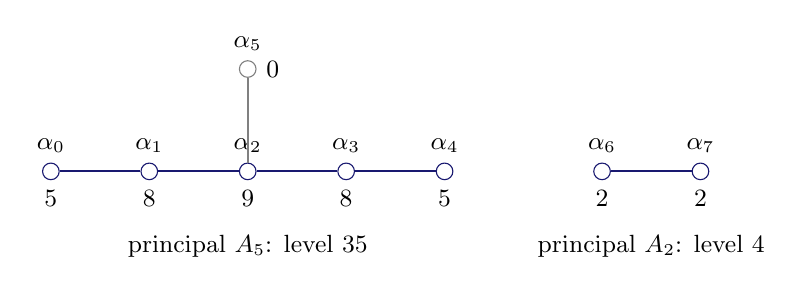
\begin{tikzpicture}[
 root/.style={circle,draw=MidnightBlue,fill=white,inner sep=0pt,minimum size=6pt},
 every label/.style={font=\small},
 line/.style={thick,MidnightBlue}
]
\foreach \i/\c in {0/5,1/8,2/9,3/8,4/5}{
 \node[root,label=above:{$\alpha_{\i}$},label=below:{$\c$}] (a\i) at (\i*1.25,0) {};
}
\node[root,draw=gray,label=above:{$\alpha_5$},label=right:{$0$}] (a5) at (2.5,1.3) {};
\node[root,label=above:{$\alpha_6$},label=below:{$2$}] (a6) at (7,0) {};
\node[root,label=above:{$\alpha_7$},label=below:{$2$}] (a7) at (8.25,0) {};
\foreach \i/\j in {0/1,1/2,2/3,3/4,6/7}{\draw[line] (a\i)--(a\j);}
\draw[thick,gray] (a2)--(a5);
\node[font=\small] at (2.5,-0.95) {principal $A_5$: level $35$};
\node[font=\small] at (7.625,-0.95) {principal $A_2$: level $4$};
\end{tikzpicture}

\caption{The $E_6\oplus A_2$ root diagram in the chosen numbering.
The integers below or beside the nodes are the coefficients
$c_i$ of the right Cartan $h=\sum_i c_i\alpha_i$. The nonzero
nodes form $A_5\oplus A_2$, whose principal triples combine
diagonally to give level $39$.}
\label{fig:c-principal-diagram}
\end{figure}

For a level-$k$ triple the Sugawara vector is
\begin{equation}\label{eq:c-sugawara}
 \omega_k=\frac1{2(k+2)}
 \left(\frac12H_{(-1)}H+E_{(-1)}F+F_{(-1)}E\right),
 \qquad c_k=\frac{3k}{k+2}.
\end{equation}
Thus the two current factors account for
\[
 c_K=1+\frac{117}{41}=\frac{158}{41}.
\]
They account for less than half of the ambient central charge eight.
The complementary stress has charge $170/41$. The desired algebra
will contain more than its affine currents.

\section{The exceptional field and the transported positive form}
\index{PCT involution!transported lattice form}

Put
\[
 a=(0,0,0,0,0,-1,1,1),\quad
 b=(0,0,0,1,1,-1,0,0),\quad
 c=(1,1,0,0,0,-1,0,0),
\]
and define
\begin{equation}\label{eq:c-u}
 u=e^a+\frac{\sqrt{13}+3\sqrt{-3}}{20}e^b
       +\frac{\sqrt{13}-3\sqrt{-3}}{20}e^c.
\end{equation}
Each momentum has squared norm four. All three terms therefore have weight two.
Their Cartan weights are $(1,13)$, and substitution in the lattice
product formula shows that the raising zero modes annihilate the
displayed linear combination. Consequently $u$ is a highest vector of
current representation dimensions $(2,14)$.

\begin{example}[The three momenta are already highest vectors]
The Gram matrix makes the preceding assertions short calculations:
\[
 Ga=\begin{pmatrix}0\\0\\1\\0\\0\\-2\\1\\1\end{pmatrix},
 \quad
 Gb=\begin{pmatrix}0\\0\\0\\1\\1\\-2\\0\\0\end{pmatrix},
 \quad
 Gc=\begin{pmatrix}1\\1\\0\\0\\0\\-2\\0\\0\end{pmatrix}.
\]
Taking coordinate dot products gives
$a^2=b^2=c^2=4$, all three pairwise inner products equal to
two, and
\[
 (\ell,a)=(\ell,b)=(\ell,c)=1,\qquad
 (h,a)=(h,b)=(h,c)=13.
\]
Every displayed pairing with a simple root occurring in $E_R$
is nonnegative; the only negative entry is at the omitted node
$5$. The exponential product then has no $z^{-1}$ term.
Thus $E_R{}_{(0)}$ kills each exponential separately.
The pairing with $\ell$ is also positive, so $E_L{}_{(0)}$
kills each separately. Their linear span is already a
three-dimensional space of highest vectors with the same charges.
Highest-weight conditions alone therefore leave their relative
coefficients undetermined. The special choice in
\eqref{eq:c-u} is selected by the further product identities.
\end{example}

The field is not chosen by demanding only its weight and Cartan charges.
The relative coefficients matter in subsequent products. In a positive
orthonormal momentum convention, the same vector is proportional to
\[
 e^a+\zeta e^b+\overline\zeta e^c,
 \qquad \zeta=\frac{\sqrt{13}+3i\sqrt3}{\sqrt{40}},
 \qquad |\zeta|^2=\frac{13+27}{40}=1.
\]
There is no free continuous phase in the stated construction. The
special phase is a concrete local datum, rather than a consequence of
the fusion rule $d^2=1+3d$ alone.

Why are the coefficients in \eqref{eq:c-u} not all of absolute value
one? The current formulas use a convenient nonunitary torus gauge.
Coordinate changes of this sort are legitimate, provided the positive
form is transported with them.

Let $\widetilde c=(5,8,9,8,5,1,2,2)$ and let $g$ fix the oscillators
and act on momenta by
\[
 g(e^\beta)=\prod_i\widetilde c_i^{-\beta_i/2}e^\beta.
\]
If $\theta$ is the ordinary lattice PCT operation, use
$\theta_g=g\theta g^{-1}$ and
$\langle v,w\rangle_g=\langle g^{-1}v,g^{-1}w\rangle$.
The form remains positive. In the explicit formula take the $h_i$
in the real lattice Cartan and extend antilinearly to complex coefficients:
\begin{equation}\label{eq:c-pct}
 \theta_g\bigl(h_1(-n_1)\cdots h_r(-n_r)e^\beta\bigr)
 =(-1)^r\prod_i\widetilde c_i^{\beta_i}
               h_1(-n_1)\cdots h_r(-n_r)e^{-\beta},
\end{equation}
with antilinear action on scalar coefficients. The factors on opposite
momenta cancel when the operation is applied twice.

\begin{example}[A large normalization with a small meaning]
For the left root,
$\prod_i\widetilde c_i^{\ell_i}=8640^{-2}$. Hence
$\theta_g(E_L)=-F_L/8640^2$. The root vectors have unequal coordinate
norms even though they span the ordinary compact level-one current
algebra. This is why a later compact diagonal current is
$8640E_L+E_R$, paired with $F_L/8640+F_R$, rather than the raw sum
$E_L+E_R$. Positivity is a statement about the transported form, not
about the apparent size of coordinates.
\end{example}

The positive real torus character extends from $E_6\oplus A_2$ to
the common real Cartan space, and hence to its $E_8$ overlattice.
The entire tower can therefore be discussed in one positive convention.

\begin{example}[The 28 states generated by one highest field]
\label{ex:c-current-multiplet}
\index{current multiplet}\index{internal spin}
We can now see an ordinary finite-dimensional representation inside the
vertex algebra, including its positive normalization. Work with the
compact zero-mode operators
\[
 e_L=8640E_L{}_{(0)},\qquad f_L=\frac{F_L{}_{(0)}}{8640},
 \qquad e_R=E_R{}_{(0)},\qquad f_R=F_R{}_{(0)}.
\]
The transported form gives $e_L^\dagger=f_L$ and
$e_R^\dagger=f_R$. The two Cartan zero modes are self-adjoint.
For either internal label, $[e,f]=H_{(0)}$,
$[H_{(0)},e]=2e$, and $[H_{(0)},f]=-2f$; operators with different
internal labels commute. These are two copies of the usual compact
$\mathfrak{sl}_2$ representation problem. Both act on holomorphic
fields: the subscripts $L,R$ here do not denote physical chirality.

First normalize the highest vector $u$. Distinct lattice momenta are
orthogonal, and the transported squared norms are
\[
 \|e^a\|_g^2=4,\qquad \|e^b\|_g^2=40,
 \qquad \|e^c\|_g^2=40.
\]
The two nontrivial coefficients in \eqref{eq:c-u} have squared modulus
$(13+27)/400=1/10$. Consequently
\[
 \|u\|_g^2=4+\frac{40}{10}+\frac{40}{10}=12.
\]
The already verified highest-vector conditions read
\[
 e_Lu=e_Ru=0,\qquad H_L{}_{(0)}u=u,
 \qquad H_R{}_{(0)}u=13u.
\]

Recall the lowering calculation for one copy of $\mathfrak{sl}_2$.
If $ev=0$ and $H_{(0)}v=mv$, commuting $e$ through $q$ lowering
operators gives
\[
 ef^qv=q(m-q+1)f^{q-1}v.
\]
For example, the coefficient is the sum
$m+(m-2)+\cdots+(m-2(q-1))=q(m-q+1)$.
Taking the inner product and using $f^\dagger=e$ proves the recursion
\[
 \|f^qv\|^2=q(m-q+1)\|f^{q-1}v\|^2,
 \qquad
 \|f^qv\|^2=q!\,\frac{m!}{(m-q)!}\|v\|^2
 \quad(0\le q\le m).
\]
Every vector in this range is nonzero. At $q=m+1$ the same recursion
gives zero norm, so positivity gives $f^{m+1}v=0$.

Apply this calculation to the two commuting copies with $m_L=1$ and
$m_R=13$. Their joint lowered vectors are
\[
 u_{r,s}=f_L^r f_R^s u,
 \qquad r=0,1,\quad s=0,1,\ldots,13.
\]
Their squared norms and Cartan weights are
\begin{align*}
 \|u_{r,s}\|_g^2&=12\,s!\,\frac{13!}{(13-s)!},\\
 (H_L{}_{(0)},H_R{}_{(0)})u_{r,s}
   &=(1-2r,\,13-2s)u_{r,s}.
\end{align*}
Here the first equality has no extra $r$ factor because both nonzero
vectors in a highest-weight-one representation have the same norm.
The 28 pairs of eigenvalues are distinct. Self-adjointness therefore
makes these vectors mutually orthogonal, and an orthonormal basis is
\begin{equation}\label{eq:c-current-multiplet-basis}
 \widehat u_{r,s}
 =\sqrt{\frac{(13-s)!}{12\,s!\,13!}}\,f_L^r f_R^s u.
\end{equation}
In this basis the familiar angular-momentum coefficients appear:
\begin{align*}
 f_L\widehat u_{0,s}&=\widehat u_{1,s},
 &f_L\widehat u_{1,s}&=0,\\
 f_R\widehat u_{r,s}
   &=\sqrt{(s+1)(13-s)}\,\widehat u_{r,s+1},
 &e_R\widehat u_{r,s}
   &=\sqrt{s(14-s)}\,\widehat u_{r,s-1}.
\end{align*}
At an endpoint the corresponding coefficient is zero. The action of
$e_L$ reverses the nonzero $f_L$ arrow. Reordering any word in the
zero modes moves raising operators to the right, where they kill
$u$, and reduces Cartan operators to their eigenvalues. Thus the
cyclic zero-mode representation is exactly this 28-dimensional space,
the irreducible tensor product of internal spins $1/2$ and $13/2$.

These lowering operations do not create Virasoro descendants.
Each exponential in $u$ is a primary of ambient conformal weight two.
For a weight-one primary current $J$, the mode relation
$[L_n,J_{(0)}]=0$ holds for every $n$. Hence
\[
 L_0u_{r,s}=2u_{r,s},\qquad L_nu_{r,s}=0\quad(n>0).
\]
All 28 vectors are weight-two Virasoro-primary components of one
internal current multiplet. The affine levels $1,39$, the internal
highest weights $1,13$, and the conformal weight $2$ measure different
things. This argument concerns current zero modes; it does not by
itself assert annihilation by every positive affine mode.
That stronger condition can be checked separately here. Each root
$\pm\ell$ or $\pm\alpha_i$ occurring in the current triples pairs
with $a,b,c$ in $\{-1,0,1\}$. Their exponential OPEs therefore have
no pole of order two or higher, so $J_{(n)}u=0$ for $n\geq1$ for
each exponential current $J$. The positive Heisenberg modes also kill
the pure exponentials. Together with $e_Lu=e_Ru=0$, these identities
prove that $u$ is an affine highest vector. They use its actual
lattice OPEs, beyond the two Cartan eigenvalues.

Finally, a three-dimensional space of available highest vectors is
not a three-dimensional multiplet. It is a multiplicity space:
choosing one highest vector selects one copy of the irreducible
28-dimensional representation. The particular line spanned by $u$
is selected by its product identities. Cartan charges alone do not
show that the PCT conjugate $\theta_g(u)$ belongs to this same cyclic
copy; PCT stability remains a separate finite construction input.
\end{example}

\section{What has actually been defined?}

We now define the object of interest:
\begin{equation}\label{eq:c-U-definition}
 U=\langle K,\omega_B,u\rangle\subset B.
\end{equation}
The angle brackets mean the smallest vertex subalgebra containing the
listed states, closed under every mode. It is an actual algebra, not
an abstract presentation whose Jacobi identities remain to be solved.
It has the ambient stress because $\omega_B$ was explicitly included.
The finite construction verifies PCT stability of the generated fields;
the induced positive form then makes $U$ a unitary VOA of CFT type.

At this point one has \emph{not} proved $U\ne B$. This is the subtle
question that motivates the next chapter. Iterated products of a few
fields can eventually generate all ambient currents, even if the first
several spaces look much smaller.

\begin{constructioninput}[Initial generated spaces]
In the fixed lattice realization, closure of the original generators
by the stated current and weight-two products constructs a PCT-stable
space $S_2\subset U_2$ of dimension $120$. It consists of $22$ affine
vacuum states, two neutral stresses, and current multiplets
\[
 (1,5),(1,9),(1,9),(1,13),(2,2),(2,6),(2,8),(2,14).
\]
The entries denote dimensions, so the multiplets contribute
$5+9+9+13+4+12+16+28=96$ states. The generated grade-three space
$S_3$ has dimension $956$, and its lower normal subspace has dimension
$634$. These are exact finite vector-space statements. Until closure
is established, they do not assert $S_i=U_i$.
\end{constructioninput}

There is a useful hand check of the number $22$. A universal affine
$\mathfrak{sl}_2$ vacuum module has three derivative states and six
symmetric two-current states at weight two, hence nine. At level one
the five-dimensional spin-two null multiplet is removed, leaving four.
The level-$39$ factor still has nine at that grade. The mixed products
contribute $3\cdot3=9$, giving $4+9+9=22$.

This calculation illustrates the correct division of labor. Small
dimension checks explain why a finite record is plausible and teach
its representation content. They do not replace the exact membership
and product identities that identify the stated vectors with the
algebra generated by \eqref{eq:c-U-definition}.

\section{The remaining construction as a chain of implications}

The ambient lattice has solved the existence and associativity
problem for the generated fields. The remaining claims have
different inputs. The following table is a guide to the argument,
not an additional assumption that all its conclusions hold.

\begin{longtable}{@{}>{\raggedright\arraybackslash}p{0.27\textwidth}p{0.69\textwidth}@{}}
\toprule
Claim to establish & Input and role in the construction\\
\midrule
\endhead
The algebra is proper. &
The finite mode identities and recursive closure theorem of
Chapter~\ref{ch:finite_closure} show that no extra currents
appear at a later stage of generation. In particular,
$U_1\cong\mathfrak{sl}_2\oplus\mathfrak{sl}_2$ has dimension six.\\[5pt]
All modules are controlled. &
The parafermion and lattice cores of Chapter~\ref{ch:factors}
give a positive conformal-vector identity.
Chapter~\ref{ch:regularity} uses it for $C_2$-cofiniteness and
the splitting argument that yields rationality.
The standard rationality--regularity implication then applies.\\[5pt]
The boundary ring is the Haagerup ring. &
Finite module tops, extension branching, and twist moments
constrain the boundary category in Chapter~\ref{ch:branching}.
They determine its fusion ring and the modular-data target.
Identifying its unitary tensor structure uses the later
positivity step.\\[5pt]
Every sector and fusion pairing is positive. &
Chapter~\ref{ch:unitarity} compares actual modules and bounded
field insertions with conformal-net sectors. Vacuum positivity
is upgraded first to strong and then to complete unitarity.
Unitary classification identifies the original boundary category
as $\HH_2$ or $\HH_3$, and its center as their common
Haagerup center.\\[5pt]
The characters are determined. &
Chapter~\ref{ch:characters} combines the resulting modular
representation with the allowed leading powers and their
coefficients. Uniqueness determines the vector of traces.
This step counts states; it does not choose extension
multiplication.\\[5pt]
There are full local theories. &
Chapters~\ref{ch:full_theories} and \ref{ch:sewing} apply rational
sewing to the diagonal pairing and to a selected canonical
$\HH_3$ extension algebra. The selected holomorphic extension
is isomorphic to $V_{E_8}$, with its specified boundary category.\\
\bottomrule
\end{longtable}

This order also explains why replacing the defining field $u$ by a
plausible field of the same weight is not a harmless variation.
The new field still generates a genuine subalgebra of the ambient
lattice VOA. It need not satisfy the finite closure, core, or
branching identities that drive the rest of the argument.

\section{Exercises}

\begin{exercise}\label{ex:c-lattice-1}
Use the cocycle formula to prove the commutator and opposite-momentum
identities immediately following \eqref{eq:c-lattice-cocycle}. Explain
where evenness of the lattice is used.

\par\smallskip\noindent{\footnotesize\normalfont
\hyperref[sol:ex:c-lattice-1]{Solution on page~\pageref*{sol:ex:c-lattice-1}.}}\par
\end{exercise}
\begin{exercise}\label{ex:c-lattice-2}
Starting from \eqref{eq:c-lattice-product}, compute all singular terms
in $Y(e^a,z)e^{-a}$ for $(a,a)=4$. Identify the weights of their
coefficients and compare with the mode weight rule.

\par\smallskip\noindent{\footnotesize\normalfont
\hyperref[sol:ex:c-lattice-2]{Solution on page~\pageref*{sol:ex:c-lattice-2}.}}\par
\end{exercise}
\begin{exercise}\label{ex:c-lattice-3}
For $\mathfrak{sl}_2$ at level $k$, the affine highest weight $r$ has
Sugawara weight $r(r+2)/(4(k+2))$. Compute the affine weight of $u$
from its labels $(1,13)$ at levels $(1,39)$, and find its remaining
weight under $\omega_B-\omega_K$.

\par\smallskip\noindent{\footnotesize\normalfont
\hyperref[sol:ex:c-lattice-3]{Solution on page~\pageref*{sol:ex:c-lattice-3}.}}\par
\end{exercise}
\begin{exercise}\label{ex:c-lattice-4}
Verify directly that $\theta_g^2=1$ and that the form transported by
$g$ is positive. Why would ordinary coefficient conjugation fail to
give the correct adjoint of $E_R$ in the displayed gauge?

\par\smallskip\noindent{\footnotesize\normalfont
\hyperref[sol:ex:c-lattice-4]{Solution on page~\pageref*{sol:ex:c-lattice-4}.}}\par
\end{exercise}
\begin{exercise}\label{ex:c-lattice-5}
Explain why an even overlattice obtained by adjoining an isotropic
subgroup $A\subset L^*/L$ has determinant $\det(L)/|A|^2$. Apply
the result to $E_6\oplus A_2$.

\par\smallskip\noindent{\footnotesize\normalfont
\hyperref[sol:ex:c-lattice-5]{Solution on page~\pageref*{sol:ex:c-lattice-5}.}}\par
\end{exercise}
